\documentclass[11pt,a4paper]{article}
\usepackage[margin=2cm]{geometry}
\usepackage{graphicx}
\usepackage{amsmath,amssymb}
\usepackage{enumitem}
\usepackage{xcolor}
\usepackage{tcolorbox}
\usepackage{booktabs}
\usepackage{hyperref}
\usepackage{fancyhdr}

\definecolor{qcolor}{HTML}{1A5276}
\definecolor{acolor}{HTML}{196F3D}
\definecolor{boxbg}{HTML}{EBF5FB}
\definecolor{ansbox}{HTML}{EAFAF1}
\definecolor{tipbox}{HTML}{FEF9E7}

\tcbset{
    qbox/.style={colback=boxbg, colframe=qcolor, coltitle=white, fonttitle=\bfseries, coltext=black, left=4pt, right=4pt, top=4pt, bottom=4pt, boxrule=0.8pt, arc=3pt},
    abox/.style={colback=ansbox, colframe=acolor, coltitle=white, fonttitle=\bfseries, coltext=black, left=4pt, right=4pt, top=4pt, bottom=4pt, boxrule=0.5pt, arc=3pt},
    tipbox/.style={colback=tipbox, colframe=orange!70!black, fonttitle=\bfseries, left=4pt, right=4pt, top=4pt, bottom=4pt, boxrule=0.5pt, arc=3pt}
}

\newcounter{qcounter}
\setcounter{qcounter}{55}
\newcommand{\vq}[1]{\stepcounter{qcounter}\begin{tcolorbox}[qbox, title=Q\theqcounter]#1\end{tcolorbox}}
\newcommand{\va}[1]{\begin{tcolorbox}[abox, title=Answer]#1\end{tcolorbox}\vspace{6pt}}

\pagestyle{fancy}
\fancyhf{}
\fancyhead[L]{\small\textbf{TFML Viva Prep — Part 3}}
\fancyhead[R]{\small CS6302E | Winter 2026}
\fancyfoot[C]{\thepage}

\title{\textbf{TFML Assignment Viva — Question Bank}\\[4pt]\Large Part 3: Architecture Search, Sample Complexity \& Theory}
\author{CS6302E — Theoretical Foundations of Machine Learning}
\date{NIT Calicut | Winter 2026}

\begin{document}
\maketitle
\tableofcontents
\newpage

%=============================================================================
\section{Architecture Search (Part e)}
%=============================================================================

\vq{How did you conduct the architecture search?}
\va{
\begin{center}
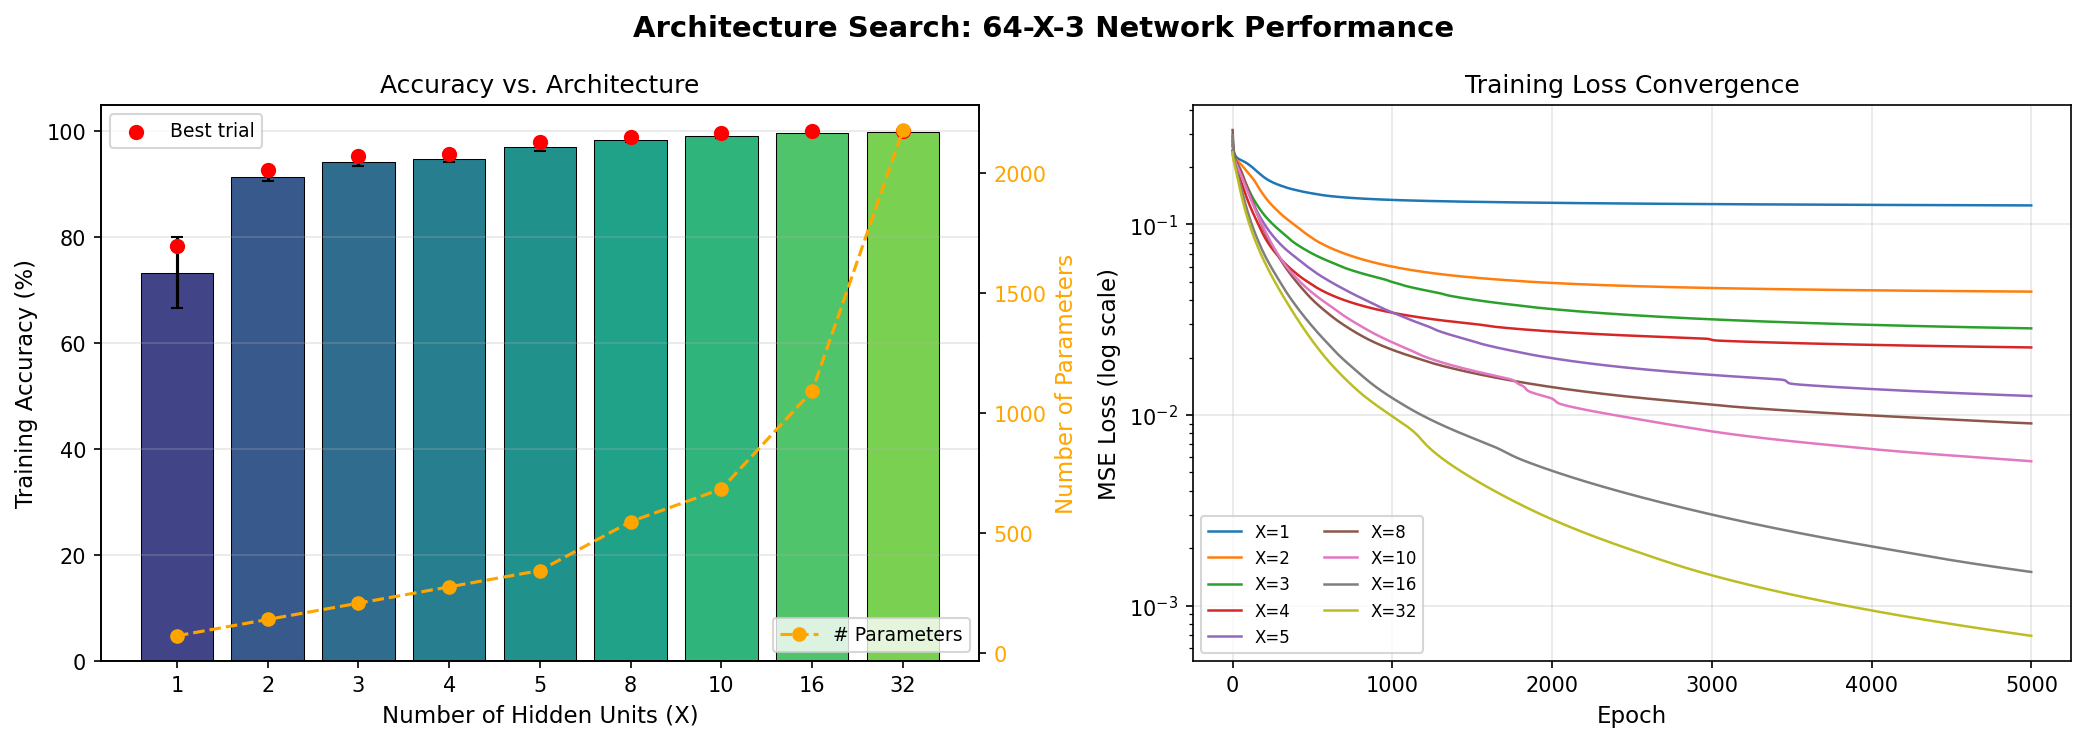
\includegraphics[width=0.90\textwidth]{architecture_search.png}
\end{center}
Tested \textbf{64-X-3 architectures} with $X \in \{1, 2, 3, 4, 5, 8, 10, 16, 32\}$. For each, \textbf{5 trials} with different random seeds. Each trained for 5000 epochs (lr=0.5, full-batch). Left: mean accuracy with error bars + parameter count. Right: loss convergence curves.
}

\vq{What happens with X=1 (only 1 hidden neuron)?}
\va{$X=1$ achieves only $\sim$\textbf{78\%} accuracy with high variance. A single hidden neuron creates only \textbf{one linear boundary} in 64D space, producing 2 regions. For 3 classes, you need at least 2 boundaries. $X=1$ can at best separate one class from the other two.}

\vq{Why does X=2 still underperform?}
\va{$X=2$ maps inputs to a \textbf{2D hidden space}. While 2 neurons can theoretically create enough boundaries for 3 classes, the 2D embedding must perfectly separate all 3 noisy clusters — geometrically difficult. Accuracy plateaus $\sim$92\% with high initialization sensitivity (high variance).}

\vq{Why is X=3 the ``minimal viable'' architecture?}
\va{With 3 hidden neurons, inputs map to a \textbf{3D hidden space}. Each neuron can serve as a dedicated feature detector for one class. The output layer has a full-rank $3\times 3$ weight matrix. This is the \textbf{minimum dimensionality} for reliable 3-class separation.}

\vq{What is the ``sweet spot'' for X and why?}
\va{The sweet spot is $X = 5$ to $X = 10$, achieving $\geq$97\% accuracy consistently with low variance. Additional neurons beyond 3 provide:
\begin{itemize}[nosep]
    \item \textbf{Redundancy}: Multiple neurons detect the same feature, improving robustness
    \item \textbf{Richer feature space}: More nuanced discriminating features
    \item \textbf{Faster convergence}: More degrees of freedom for optimization
\end{itemize}
Beyond $X=10$, gains are marginal (noise-limited).
}

\vq{Describe the accuracy convergence plot for different architectures.}
\va{
\begin{center}
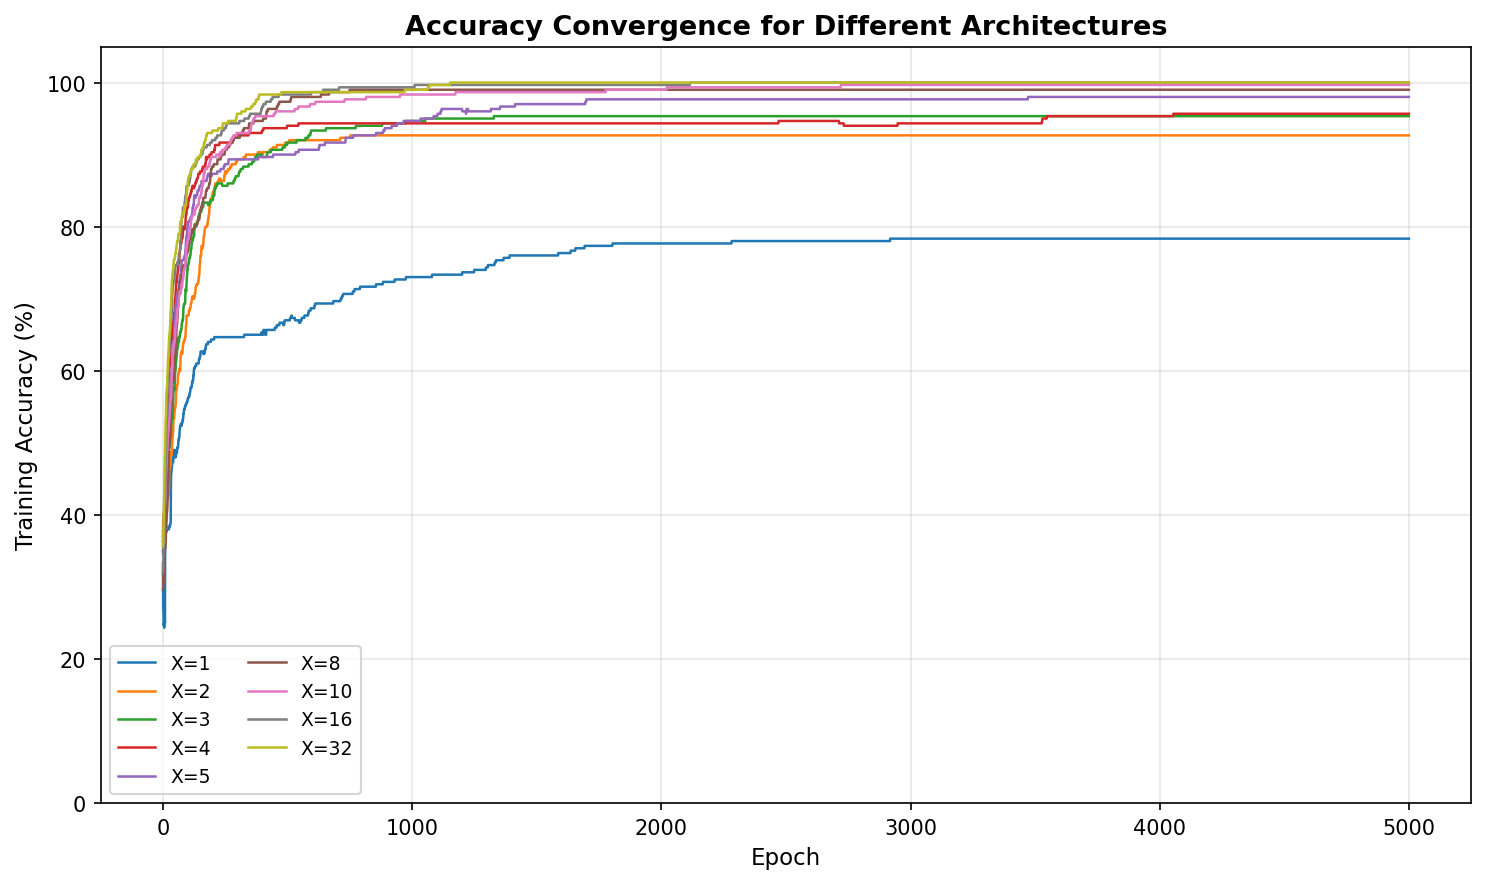
\includegraphics[width=0.75\textwidth]{accuracy_convergence.png}
\end{center}
\begin{itemize}[nosep]
    \item $X=1$: Slowest, plateaus at $\sim$78\% — never achieves high accuracy
    \item $X=2$: Plateaus at $\sim$92\% with slow climb
    \item $X=3$ to $X=5$: Rapid initial learning ($>$90\% within 200--500 epochs)
    \item $X=8, 16, 32$: Fastest convergence, reaching 99--100\% within 500--1000 epochs
    \item \textbf{Key}: More hidden units $\to$ faster convergence AND higher final accuracy, with diminishing returns
\end{itemize}
}

\vq{What does the training loss convergence (right panel) tell you?}
\va{
\begin{itemize}[nosep]
    \item $X=1$: Loss plateaus at $\sim$0.13 — the model \textbf{underfits}
    \item $X=32$: Loss drops to $\sim$0.001 — enough capacity for near-perfect fit
    \item Convergence \textbf{rate increases} with more hidden units — smoother loss landscapes
    \item All curves monotonically decreasing: full-batch GD with lr=0.5 is stable for all architectures
\end{itemize}
}

\vq{How does the number of parameters grow with X?}
\va{For 64-X-3: Parameters $= (64 \times X + X) + (X \times 3 + 3) = \mathbf{67X + 3}$

\begin{center}
\begin{tabular}{lcccccc}
\toprule
$X$ & 3 & 5 & 10 & 16 & 32 \\
\midrule
Params & 207 & 338 & 673 & 1075 & 2147 \\
\bottomrule
\end{tabular}
\end{center}
Growth is \textbf{linear in $X$}. The orange dashed line in the plot shows this overlaid with accuracy bars.
}

\vq{Is there overfitting with X=32?}
\va{On \textbf{training set}, $X=32$ achieves $\sim$100\%. To assess overfitting, compare with test performance. The sample complexity analysis shows that with 100 training samples per class, even $X=16$ generalizes reasonably. True overfitting = high training accuracy but poor test accuracy. The gap between training ($\sim$100\%) and test ($\sim$63\%) accuracy for large $X$ does suggest some overfitting.}

%=============================================================================
\section{Sample Complexity Analysis (Part e)}
%=============================================================================

\vq{How did you study sample complexity?}
\va{
\begin{center}
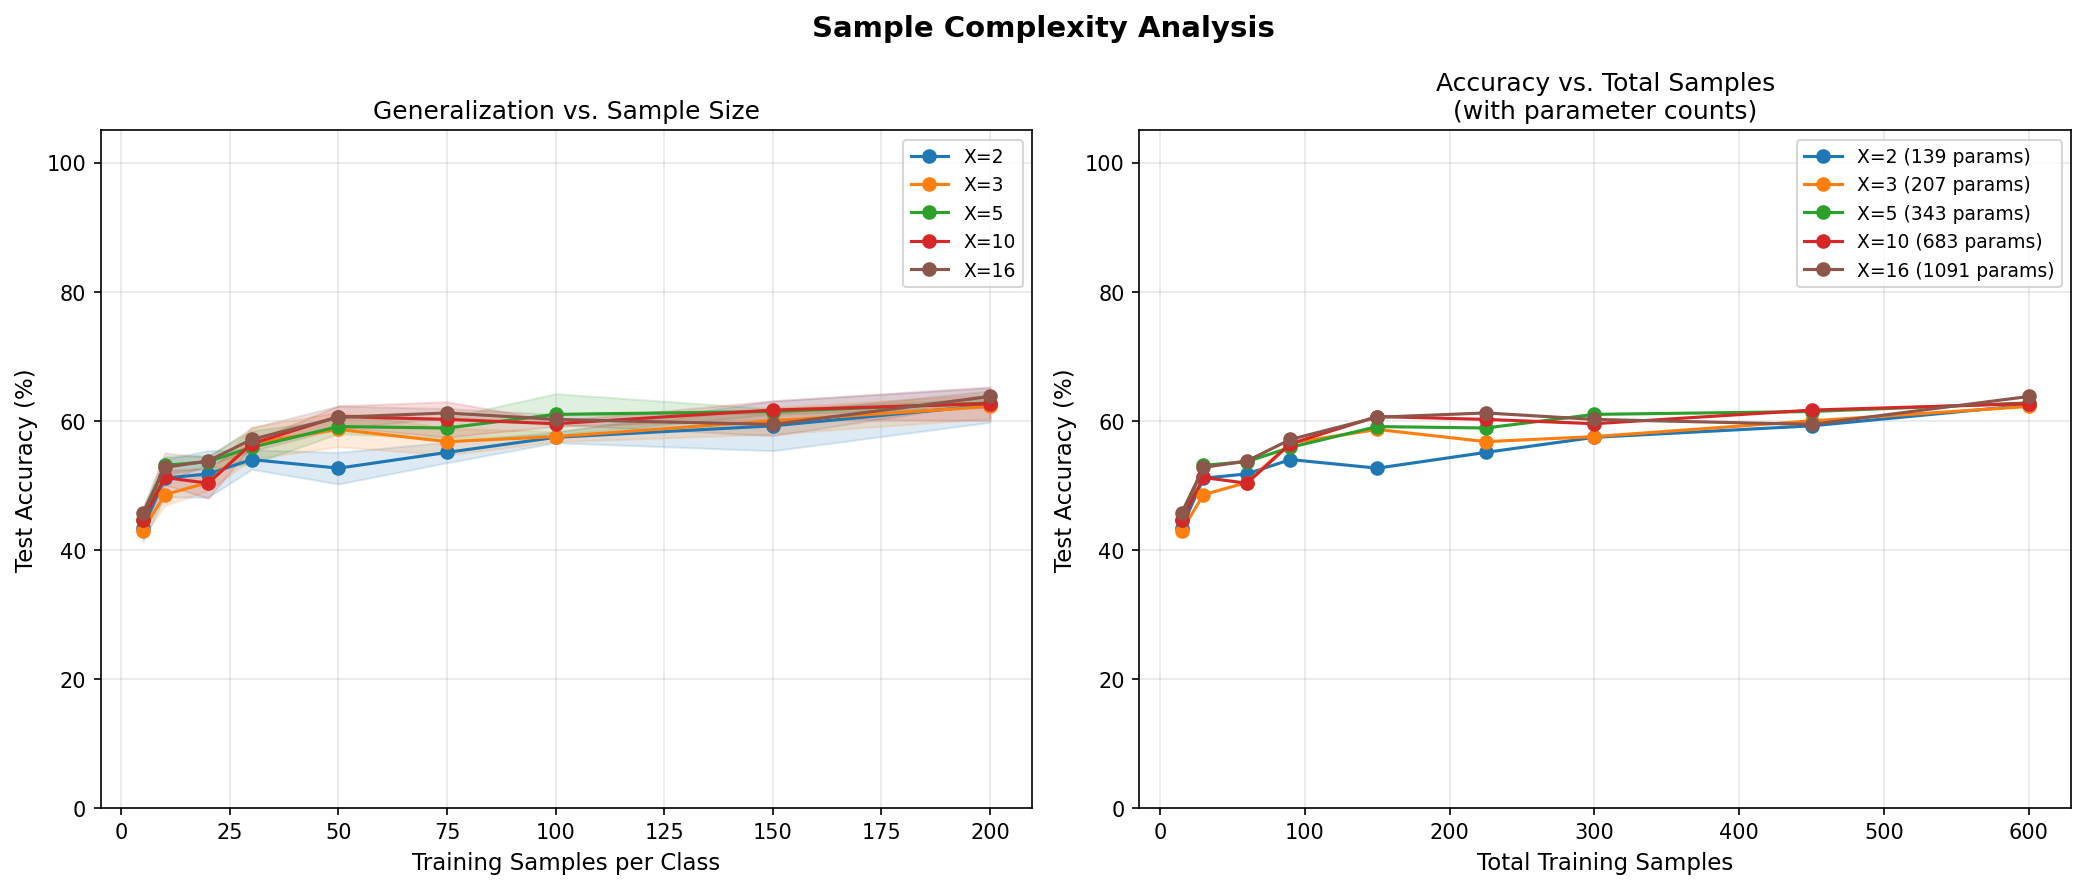
\includegraphics[width=0.90\textwidth]{sample_complexity.png}
\end{center}
Varied \textbf{training samples per class} from 5 to 200 and measured \textbf{test accuracy} on 300 separate test samples. Done for $X \in \{2, 3, 5, 10, 16\}$. Left: per-class samples. Right: total samples with parameter counts.
}

\vq{What happens with very few training samples (5--10 per class)?}
\va{All architectures struggle ($\sim$43--50\% test accuracy, barely above random 33\%). With so few samples, the network \textbf{memorizes specific noise patterns} rather than learning templates. The noise doesn't average out, so signal remains buried.}

\vq{Describe the general trend in the sample complexity curves.}
\va{
\begin{enumerate}[nosep]
    \item \textbf{Rapid improvement} from 5$\to$30 samples ($\sim$45\% to $\sim$55--60\%)
    \item \textbf{Diminishing returns} beyond 50 samples — accuracy plateaus at 60--64\%
    \item \textbf{More complex models} (higher $X$) achieve slightly higher final accuracy
    \item The \textbf{plateau} at 60--65\% is due to the Bayes error imposed by extreme noise
\end{enumerate}
}

\vq{Why do simpler architectures plateau at lower accuracy than complex ones?}
\va{Simpler architectures have a \textbf{lower capacity ceiling}. $X=2$ (139 params) maps to a 2D hidden space, limiting its ability to separate noisy clusters. $X=16$ (1091 params) has a much richer \textbf{hypothesis space} and can learn more nuanced features, achieving higher accuracy with enough data.}

\vq{What does the shaded region in the left panel represent?}
\va{The \textbf{variance across multiple trials} (confidence interval). Wider shading = more variance = less reliable. At low sample counts, shading is wide (unstable learning). At high sample counts, shading narrows (consistent performance). This shows the \textbf{stability} of learning improves with more data.}

\vq{Why does test accuracy plateau at $\sim$60--65\% instead of 90\%+?}
\va{
\begin{enumerate}[nosep]
    \item Test samples have \textbf{different noise} — model must generalize
    \item Many test samples are \textbf{intrinsically ambiguous} at this noise level
    \item The \textbf{Bayes error rate} is high — even the optimal classifier would err frequently
    \item Model relies on \textbf{learned average features}, not memorized noise
\end{enumerate}
}

%=============================================================================
\section{VC Dimension \& Generalization Theory}
%=============================================================================

\vq{What is VC dimension and how does it relate to your network?}
\va{\textbf{VC (Vapnik-Chervonenkis) dimension} is the maximum number of points that can be \textbf{shattered} (classified in all $2^n$ possible ways) by a hypothesis class.
\begin{itemize}[nosep]
    \item For neural networks, VC dimension grows with the \textbf{number of parameters}
    \item Our 64-3-3 network: $d_{VC} \approx O(207)$
    \item Higher $d_{VC}$ = can fit more complex patterns but needs more data to generalize
\end{itemize}
}

\vq{How does VC dimension connect to your sample complexity results?}
\va{Statistical learning theory: for good generalization, $n \geq O(d_{VC} / \varepsilon)$.

Our results confirm: networks with more parameters (higher $d_{VC}$) need more training samples. $X=16$ (1091 params) requires $\sim$100+ samples/class, while $X=3$ (207 params) reaches near-peak with $\sim$30--50 samples.}

\vq{What is the bias-variance tradeoff and how does it manifest?}
\va{
\begin{itemize}[nosep]
    \item \textbf{Bias}: Error from being too simple (underfitting). $X=1$ has high bias.
    \item \textbf{Variance}: Error from being too sensitive to training data (overfitting). $X=32$ has potentially high variance.
    \item \textbf{Tradeoff}: As complexity increases, bias $\downarrow$ but variance can $\uparrow$.
\end{itemize}
In our results: $X=1$--$2$: high bias, low variance $\to$ consistently poor. $X=5$--$10$: low bias, moderate variance $\to$ sweet spot. $X=16$--$32$: very low bias, potentially higher variance.
}

\vq{What does the PAC learning framework say about your problem?}
\va{PAC asks: ``How many samples to learn with probability $\geq 1-\delta$ to accuracy $\geq 1-\varepsilon$?''
$$n \geq \frac{1}{\varepsilon}\left(d_{VC} \cdot \ln\frac{1}{\varepsilon} + \ln\frac{1}{\delta}\right)$$
For $d_{VC} \approx 207$, $\varepsilon=0.05$, $\delta=0.05$: $n \approx 12{,}000$. Our 300 samples are well below this \textbf{worst-case bound}, but the bound is loose — our problem has more structure.
}

\vq{What is the difference between training error and generalization error?}
\va{
\begin{itemize}[nosep]
    \item \textbf{Training error}: Error on training data ($\sim$6\% from confusion matrix)
    \item \textbf{Generalization error}: Expected error on \textbf{unseen data} from same distribution
    \item \textbf{Gap} = Generalization error $-$ Training error
\end{itemize}
Our sample complexity shows: training accuracy can reach $\sim$100\% ($X=32$), but test accuracy plateaus at $\sim$63\%. The gap is large for high-capacity models on small datasets.
}

\vq{What is structural risk minimization (SRM)?}
\va{SRM balances:
\begin{enumerate}[nosep]
    \item \textbf{Empirical risk} (training error): decreases with complexity
    \item \textbf{Complexity penalty} (related to $d_{VC}$): increases with complexity
\end{enumerate}
Optimal model minimizes: total risk $=$ empirical risk $+$ complexity term.

Our architecture search is SRM in practice: $X=1$--$2$ have high empirical risk (underfit); $X=32$ has low empirical risk but high complexity; $X=5$--$10$ is the optimal balance.
}

\vq{Can your neural network learn any Boolean function of the 64 inputs?}
\va{With sigmoid activations and enough hidden units, the network can \textbf{approximate any continuous function} (Universal Approximation Theorem). However, the theorem guarantees \textbf{representational capacity} only — not learnability or sample efficiency. In practice, gradient descent may not find optimal weights, and limited data may prevent generalization.}

\begin{tcolorbox}[tipbox, title=\textbf{End of Part 3}]
\textbf{23 questions (Q56--Q78) covered.} Continue to Part 4 for implementation details, web app, and rapid-fire theory.
\end{tcolorbox}

\end{document}
